%%This is a very basic article template.
%%There is just one section and two subsections.
\documentclass{scrartcl}

\newcommand{\Botversion}{1.2.8}

\usepackage{color}

\definecolor{lightblue}{rgb}{0.9,0.95,1}
\definecolor{captionblue}{rgb}{0,0.2,0.6}

\usepackage{rotating}
\usepackage{cclic}
\usepackage{xmpincl}
\includexmp{byncsa}

\usepackage{tabularx}
\usepackage{listings}  
\usepackage{url}
\usepackage[T1]{fontenc}
\usepackage[utf8]{inputenc}
\usepackage{ngerman}
%language definition
\usepackage[ngerman]{babel}
\usepackage{ulem}
\usepackage{framed}

\newenvironment{mytab}{\par\small\tabularx}{\endtabularx} 

\definecolor{darkgrey}{rgb}{0.3,0.3,0.0}

\usepackage[pdftex, 
    colorlinks=true,
    linkcolor=darkgrey,
    filecolor=red,
    citecolor=black,
    pdftitle={BKampfBot},
    pdfauthor={georf},
    pdfsubject={BKampfBot-Dokumentation},
    pdfkeywords={Bundeskampf Bot Doku Dokumentations Bedienung},
    bookmarks, bookmarksnumbered=true, plainpages=false, pdfpagelabels]{hyperref}
\usepackage{tikz}

\definecolor{shadecolor}{rgb}{.9,.9,1}

\setlength{\parindent}{0ex}

\lstset{%
  commentstyle=\it,
  keywordstyle=\bf,
  stringstyle=\color{red},
  backgroundcolor=\color{lightblue},
  frame=single,
  basicstyle=\small\ttfamily,
  emphstyle=\bf,
}%
\lstset{literate= {Ö}{{\"O}}1 {Ä}{{\"A}}1 {Ü}{{\"U}}1 {ß}{{\ss{}}}1 {ü}{{\"u}}1 {ä}{{\"a}}1 {ö}{{\"o}}1 }

\lstnewenvironment{code}[1][]%
  {\minipage{\linewidth} 
   \lstset{basicstyle=\ttfamily\footnotesize,frame=single,#1}}
  {\endminipage}



\clubpenalty = 1000 % reduziert Schusterjungen
\widowpenalty = 1000 % reduziert Hurenkinder



\begin{document}


\begin{titlepage}
\begin{center}

\includegraphics[width=85mm]{bkampfbotlogo.png}
\\ \Large \sl {Dokumentation} \\

\vspace{25pt}
\end{center}

\tableofcontents

\end{titlepage}

\setlength{\parskip}{5pt}

\section{Hinweise zu AGB - Benutzung Verboten}
\label{verboten}
Laut den Allgemeine Geschäftsbedingungen der Spielwerk GmbH\footnote{\url{http://spielwerk.eu/index.php?option=com_content&view=article&id=90&yt_color=mint&Itemid=157}} ist die \textbf{Benutzung} dieses Programms \textbf{verboten}. Benutzt man es trotzdem, kann man \textbf{vom Spiel ausgeschlossen} werden.

Es gibt mittlerweile dazu auch ein Statement\footnote{\url{http://www.georf.de/bundeskampf-bot-version-1/\#comment-305}} von einem Administrator:

\begin{shaded}
\begin{quote}
Hallo,

    ich wünsche den Tüftlern der Bots weiterhin viel Spaß und an die Nutzer nur folgendes: Bitte wundert euch nicht, wenn eure Spielaccounts über kurz oder lang Lifetime gesperrt werden. Ihr verstoßt mit der Nutzung gegen AGB und verursacht Zusatzarbeitszeit, die wir eigentlich lieber in die Weiterentwicklung des Spieles investieren würden. Wie dem auch sein Botusing ist kein Kavaliersdelikt, kann sehr wohl von uns nachvollzogen werden und wird definitiv mit einer Komplettsperrung auf Lebenszeit geahndet.

    MfG,

    Daybreaker

    Spieladministrator Bundeskampf

\end{quote}
\end{shaded}

\section{Runterladen benötigter Dateien}
Auf der Webseite\footnote{\url{http://bundeskampf.georf.de}} kann man verschiedene Dateien runterladen. Java\footnote{\url{http://www.java.com/de/download/}} wird für die Ausführung benötigt. Für einen einfachen Betrieb braucht man dann nur zwei Dateien:
\begin{itemize}
  \item BKampfBot.jar
  \item config.json
\end{itemize}

Die \texttt{.jar}-Datei heißt auf der Webseite, wie die aktuelle Version. Zur Zeit der Dokumentation lautet der Name "\texttt{\Botversion.jar}". Man kann diesen Namen umbenennen. Beide Dateien müssen im gleichen Verzeichnis liegen.

Über das Trac\footnote{\url{https://warnow.mgvmedia.com/trac/BKampfBot/}} kann man sich den Quellcode angucken und runterladen. Diesen braucht man nur, falls man das Programm verändern möchte. Dazu sollte man beachten, dass der Code unter der Lizenz GPLv2\footnote{\url{http://www.gnu.org/licenses/gpl.html}} steht.


\section{Schnellstart Windows}
Da schon viele Windowsnutzer beim ersten Starten scheitern, habe ich eine Zip-Datei mit allen nötigen Dateien erstellt (\texttt{schnellstartWindows.zip}). Dort ist auch eine Stapelverarbeitungsdatei (\texttt{start.bat}) enthalten. Nach dem Entpacken einfach einmal diese Datei starten. Es sollte sich ein Fenster öffnen, welches erst nach Bestätigung wieder schließt. Nach dem ersten Starten sollte die Ausgabe ungefähr so aussehen:
 
\begin{code}[basicstyle=\tiny\ttfamily]
00:41 Login (meinName)
Get an error at initiation
Reason 1: Login failed
Reason 2: Something on server side changed.

If you want to report a bug, please post this:

Expected a ':' after a key at character 24
json.JSONTokener.syntaxError(JSONTokener.java:419)
json.JSONObject.<init>(JSONObject.java:212)
[...]
\end{code}

Der Login kann natürlich nicht stattfinden. Es fehlen die Logindaten in der Konfiguration. Außerdem ist der Hostname des Spiels nicht gesetzt. Diese Datei (\texttt{config.json}) ist zu öffnen zu die entsprechenden Einträge zu bearbeiten. Bei Hostname könnte man \texttt{http://www.bundeskampf.com/} eintragen, wenn man sich \hyperref[verboten]{dessen bewusst} ist, was man dort tut. 

Sollte nun ein Login möglich sein, erklärt der Rest der Dokumentation, wie man den Bot einstellt. Sollte es nicht funktionieren, bitte auch \textbf{zuerst} dieses PDF lesen und dann beschweren.

\section{Allgemeine Hinweise zum Programm}
Das Programm arbeitet über die Kommandozeile. Öffnen Sie also zuerst eine Konsole und navigieren Sie in das Verzeichnis, wohin Sie die Datei geladen haben. \footnote{Windows: \url{http://www.carpelibrum.de/tutorials/windows_konsole.pdf}}\footnote{Linux: \url{http://wiki.ubuntuusers.de/Terminal}}

 

Der allgemeine Aufruf dann sieht wie folgt aus: 

\begin{code}
eingabe# java -jar BKampfBot.jar
\end{code}

Ruft man das Programm nur mit der Hilfe auf, erschein folgendes:

\begin{code}[emph={help},basicstyle=\tiny\ttfamily]
eingabe# java -jar BKampfBot.jar --help
 ____    _  __                      __ 
|  _  \ | |/ /                     / _|
| | | | | ' / __ _ _ __ ___  _ __ | |_
| | | | |  < / _` | '_ ` _ \| '_ \|  _|
| |_| | | . \ (_| | | | | | | |_) | |
|     / |_|\_\__,_|_| |_| |_| .__/|_|
|   -<   ____        _      | |
|  _  \ |  _ \      | |     |_|
| | | | | |_) | ___ | |_
| | | | |  _ < / _ \| __|
| |_| | | |_) | (_) | |_
|_____/ |____/ \___/ \__|


BKampfBot - Version: 1.1.alpha4

Aufruf: BKampfBot.jar [Optionen]
        BKampfBot.jar [Optionen] Tag-Modi [Tag-Modi]
        BKampfBot.jar [Optionen] lotto
        BKampfBot.jar [Optionen] pins=PINARRAY
		BKampfBot.jar [Optionen] testproxy

Optionen:
  --help  -h     		Zeigt diese Hilfe an
  --config=FILE  		Nimmt FILE als Konfiguration
  --output=INT   		Setzt INT als Output-Level
  --fightAgain=INT		Setzt INT als D-Mark für erneuten Angriff

Tag-Modi:
  quiz           Tagesquiz
  los            Rubbellos
  spiel          Tagesspiel
  wein           Weinkeller
  glueck         Glücksrad

Weitere Hinweise auf http://bundeskampf.georf.de

\end{code}


\section{Ausgaben}
Das Programm erzeugt Konsolenausgaben. Dabei schreibt es in \texttt{stderr} (Fehlerausgabe) und \texttt{stdout} (Normale Ausgabe). Es gibt nun Möglichkeiten diese Ausgaben getrennt, bzw. zusammen in eine Datei umzuleiten. Dadurch kann man mehrere Stunden zurückblicken. Die Konsole speichert nur eine bestimmte Anzahl von Zeilen, die man zurück scrollen kann. Die Ausgabeumleitung ist in Windows\footnote{\url{http://support.microsoft.com/kb/110930/de}} und Linux\footnote{\url{http://www.fibel.org/linux/lfo-0.6.0/node111.html}} möglich.


\section{Konfigurationsdatei}
Normalerweise liegt die Datei \texttt{config.json} im gleichen Verzeichnis, wie das Programm. Es müssen bestimmte Angaben gemacht werden, ohne die das Programm beim Start einen Fehler ausgibt. Dazu gehören: "Benutzername", "Passwort" und "Host". Name und Passwort werden in `"' eingeschlossen und bezeichnen die Zugangsdaten. Der Host ist das Ziel jeder Anfrage. Man könnte hier zum Beispiel \texttt{http://www.bundeskampf.com/} setzen, wenn man sich \hyperref[verboten]{des AGB-Verstoßes} bewusst ist. 

"Ausgabe" bezeichnet die Menge der Ausgabe. $0 \to$ nur Fehler; $1\to$ Hinweise auf aktuelle Funktionen; $2\to$ alle Ausgaben. Diesen Wert kann man auch mittels Option \textrm{--output} gesetzt werden. Die beiden weiteren Angaben werden als Listen bezeichnet und beinhalten die Funktionen, die im Abschnitt \ref{plan} erklärt werden.

Alle Zeilen, die mit der Raute (\#) anfangen, werden nicht benutzt. Sie können also als Kommentare oder Ausklammeroperator genutzt werden.

Beispiele für Konfigurationsdateien finden Sie im Abschnitt \ref{example}.

Hier folgt eine minimale Konfigurationsdatei.

\begin{code}[language=bash]
"Benutzername":"name",
"Passwort":"geheim"
\end{code}
   
\vspace{1cm}
In der folgenden Tabelle sind alle Konfigurationsparameter aufgelistet.
   
\begin{mytab}{\textwidth}{|l|X|c|c|}
\hline
 \textbf{Name} & \textbf{Beschreibung} &  \begin{sideways} \textbf {Datentyp} \end{sideways} \\ \hline
"Benutzername" & Pflichtangabe & \texttt{String} \\ \hline
"Passwort" & Pflichtangabe & \texttt{String} \\ \hline
"Ausgabe" & Wert für die Menge der Ausgabe (0,1 oder 2) & \texttt{Int} \\ \hline
"Plan0" & Plan, wenn der Außendienst verfügbar ist & \texttt{Array} \\ \hline
"Plan1" & Plan, wenn der Außendienst nicht verfügbar ist & \texttt{Array} \\ \hline
"Angriff nochmal" & Wenn der Gewinn beim Angriff überschritten wird, wird der Gegner nochmal angegriffen & \texttt{Int} \\ \hline
"Info Pfad" & Siehe \nameref{Infopfad} & \texttt{String} \\ \hline
"Mehr Aussendienste" & Angabe, wie viele Außendienste zusätzlich mit Zwergeneinsatz gemacht werden sollen & \texttt{Int} \\ \hline
"Zeitfaktor" & Siehe \nameref{Zeitfaktor} & \texttt{Double} \\ \hline
"Useragent" & Siehe \nameref{Useragent} & \texttt{String} \\ \hline
"Vorausschauen" & Sollen die Pläne vorausschauend arbeiten (Siehe \nameref{Vorausschauen}) &  \texttt{Bool} \\ \hline
"Proxy" & Siehe \nameref{Proxy} &  \texttt{Object} \\ \hline
"Verschleiern" & Siehe \nameref{Verschleiern} &  \texttt{Bool} \\ \hline
\end{mytab}

\section{Programm-Ablaufplan}
\label{plan}
Die eigentliche Aufgabe des Programms beinhaltet das Abarbeiten eines Plans nach bestimmten Kriterien. Dieser Plan wird in der Konfigurationsdatei \\ (\texttt{config.json}) definiert. Es gibt zwei unterschiedliche Pläne, in denen einzelne Funktionen aufgerufen werden.

Der Plan 0 (in der Version 1.0 als "Außendienst verfügbar" bezeichnet) wird ausgeführt, falls man am aktuellen Tag noch einen Außendienst machen darf. Nach jedem Aufruf einer Funktion wird erneut geprüft ob noch Außendienste gemacht werden dürfen. Ist das nicht der Fall, wird in den Plan 1 übergegangen.

Der Plan 1 (in der Version 1.0 als "Kein Außendienst" bezeichnet) wird in zwei Fällen ausgeführt. Zum einen, wenn im Plan 0 keine Funktionen definiert sind, der Plan also leer ist. Zum anderen, wenn es für den aktuellen Plan keine Außen\-dienste mehr ausgeführt werden können.



Die Pläne werden in der Config in einer Aufzählung beschrieben. Zwischen ihnen müssen also immer Kommata stehen. Hier ein Beispiel:

\begin{code}[language=bash]
"Plan0":[
	{"Aussendienst":0},
	{"Aussendienst":1},
	{"Bank":0},
	{"Bank":103},
	{"Boese":0}
],
\end{code}

Wie man erkennen kann, werden die Funktionen in eckigen Klammern eingeschlossen. Nach der letzten Funktion kommt kein Kommata.

Es folgt ein Diagramm zur Erleuterung des Ablaufs der Pläne:

\resizebox{12cm}{!}{% Graphic for TeX using PGF
% Title: /home/georf/workspace/BundeskampfHilfe/flussdiagramm.dia
% Creator: Dia v0.97.1
% CreationDate: Fri Apr 29 10:11:47 2011
% For: georf
% \usepackage{tikz}
% The following commands are not supported in PSTricks at present
% We define them conditionally, so when they are implemented,
% this pgf file will use them.
\ifx\du\undefined
  \newlength{\du}
\fi
\setlength{\du}{15\unitlength}
\begin{tikzpicture}
\pgftransformxscale{1.000000}
\pgftransformyscale{-1.000000}
\definecolor{dialinecolor}{rgb}{0.000000, 0.000000, 0.000000}
\pgfsetstrokecolor{dialinecolor}
\definecolor{dialinecolor}{rgb}{1.000000, 1.000000, 1.000000}
\pgfsetfillcolor{dialinecolor}
% setfont left to latex
\definecolor{dialinecolor}{rgb}{0.000000, 0.000000, 0.000000}
\pgfsetstrokecolor{dialinecolor}
\node[anchor=west] at (15.600000\du,6.050000\du){};
\pgfsetlinewidth{0.100000\du}
\pgfsetdash{}{0pt}
\pgfsetdash{}{0pt}
\pgfsetbuttcap
{
\definecolor{dialinecolor}{rgb}{0.000000, 0.000000, 0.000000}
\pgfsetfillcolor{dialinecolor}
% was here!!!
\pgfsetarrowsend{latex}
\definecolor{dialinecolor}{rgb}{0.000000, 0.000000, 0.000000}
\pgfsetstrokecolor{dialinecolor}
\draw (16.000000\du,8.000000\du)--(16.000000\du,10.000000\du);
}
\pgfsetlinewidth{0.100000\du}
\pgfsetdash{}{0pt}
\pgfsetdash{}{0pt}
\pgfsetmiterjoin
\pgfsetbuttcap
\definecolor{dialinecolor}{rgb}{1.000000, 1.000000, 1.000000}
\pgfsetfillcolor{dialinecolor}
\fill (13.000000\du,13.000000\du)--(16.000000\du,10.000000\du)--(19.000000\du,13.000000\du)--(16.000000\du,16.000000\du)--cycle;
\definecolor{dialinecolor}{rgb}{0.000000, 0.000000, 0.000000}
\pgfsetstrokecolor{dialinecolor}
\draw (13.000000\du,13.000000\du)--(16.000000\du,10.000000\du)--(19.000000\du,13.000000\du)--(16.000000\du,16.000000\du)--cycle;
% setfont left to latex
\definecolor{dialinecolor}{rgb}{0.000000, 0.000000, 0.000000}
\pgfsetstrokecolor{dialinecolor}
\node[anchor=west] at (16.000000\du,13.000000\du){};
% setfont left to latex
\definecolor{dialinecolor}{rgb}{0.000000, 0.000000, 0.000000}
\pgfsetstrokecolor{dialinecolor}
\node at (16.000000\du,12.821250\du){Plan0};
% setfont left to latex
\definecolor{dialinecolor}{rgb}{0.000000, 0.000000, 0.000000}
\pgfsetstrokecolor{dialinecolor}
\node at (16.000000\du,13.621250\du){leer?};
\pgfsetlinewidth{0.100000\du}
\pgfsetdash{}{0pt}
\pgfsetdash{}{0pt}
\pgfsetmiterjoin
\pgfsetbuttcap
\definecolor{dialinecolor}{rgb}{1.000000, 1.000000, 1.000000}
\pgfsetfillcolor{dialinecolor}
\fill (21.000000\du,13.000000\du)--(24.000000\du,10.000000\du)--(27.000000\du,13.000000\du)--(24.000000\du,16.000000\du)--cycle;
\definecolor{dialinecolor}{rgb}{0.000000, 0.000000, 0.000000}
\pgfsetstrokecolor{dialinecolor}
\draw (21.000000\du,13.000000\du)--(24.000000\du,10.000000\du)--(27.000000\du,13.000000\du)--(24.000000\du,16.000000\du)--cycle;
% setfont left to latex
\definecolor{dialinecolor}{rgb}{0.000000, 0.000000, 0.000000}
\pgfsetstrokecolor{dialinecolor}
\node at (24.000000\du,12.821250\du){Außendienst};
% setfont left to latex
\definecolor{dialinecolor}{rgb}{0.000000, 0.000000, 0.000000}
\pgfsetstrokecolor{dialinecolor}
\node at (24.000000\du,13.621250\du){verfügbar?};
\pgfsetlinewidth{0.100000\du}
\pgfsetdash{}{0pt}
\pgfsetdash{}{0pt}
\pgfsetbuttcap
{
\definecolor{dialinecolor}{rgb}{0.000000, 0.000000, 0.000000}
\pgfsetfillcolor{dialinecolor}
% was here!!!
\pgfsetarrowsend{latex}
\definecolor{dialinecolor}{rgb}{0.000000, 0.000000, 0.000000}
\pgfsetstrokecolor{dialinecolor}
\draw (19.000000\du,13.000000\du)--(21.000000\du,13.000000\du);
}
% setfont left to latex
\definecolor{dialinecolor}{rgb}{0.000000, 0.000000, 0.000000}
\pgfsetstrokecolor{dialinecolor}
\node[anchor=west] at (19.000000\du,12.000000\du){Nein};
\pgfsetlinewidth{0.100000\du}
\pgfsetdash{}{0pt}
\pgfsetdash{}{0pt}
\pgfsetmiterjoin
\definecolor{dialinecolor}{rgb}{1.000000, 1.000000, 1.000000}
\pgfsetfillcolor{dialinecolor}
\fill (26.000000\du,17.000000\du)--(26.000000\du,19.000000\du)--(33.000000\du,19.000000\du)--(33.000000\du,17.000000\du)--cycle;
\definecolor{dialinecolor}{rgb}{0.000000, 0.000000, 0.000000}
\pgfsetstrokecolor{dialinecolor}
\draw (26.000000\du,17.000000\du)--(26.000000\du,19.000000\du)--(33.000000\du,19.000000\du)--(33.000000\du,17.000000\du)--cycle;
% setfont left to latex
\definecolor{dialinecolor}{rgb}{0.000000, 0.000000, 0.000000}
\pgfsetstrokecolor{dialinecolor}
\node at (29.500000\du,18.221250\du){Aufgaben - Plan0};
\pgfsetlinewidth{0.100000\du}
\pgfsetdash{}{0pt}
\pgfsetdash{}{0pt}
\pgfsetmiterjoin
\pgfsetbuttcap
\definecolor{dialinecolor}{rgb}{1.000000, 1.000000, 1.000000}
\pgfsetfillcolor{dialinecolor}
\fill (13.000000\du,21.000000\du)--(16.000000\du,18.000000\du)--(19.000000\du,21.000000\du)--(16.000000\du,24.000000\du)--cycle;
\definecolor{dialinecolor}{rgb}{0.000000, 0.000000, 0.000000}
\pgfsetstrokecolor{dialinecolor}
\draw (13.000000\du,21.000000\du)--(16.000000\du,18.000000\du)--(19.000000\du,21.000000\du)--(16.000000\du,24.000000\du)--cycle;
% setfont left to latex
\definecolor{dialinecolor}{rgb}{0.000000, 0.000000, 0.000000}
\pgfsetstrokecolor{dialinecolor}
\node at (16.000000\du,20.821250\du){Plan1};
% setfont left to latex
\definecolor{dialinecolor}{rgb}{0.000000, 0.000000, 0.000000}
\pgfsetstrokecolor{dialinecolor}
\node at (16.000000\du,21.621250\du){leer?};
\pgfsetlinewidth{0.100000\du}
\pgfsetdash{}{0pt}
\pgfsetdash{}{0pt}
\pgfsetbuttcap
{
\definecolor{dialinecolor}{rgb}{0.000000, 0.000000, 0.000000}
\pgfsetfillcolor{dialinecolor}
% was here!!!
\pgfsetarrowsend{latex}
\definecolor{dialinecolor}{rgb}{0.000000, 0.000000, 0.000000}
\pgfsetstrokecolor{dialinecolor}
\draw (16.000000\du,16.000000\du)--(16.000000\du,18.000000\du);
}
% setfont left to latex
\definecolor{dialinecolor}{rgb}{0.000000, 0.000000, 0.000000}
\pgfsetstrokecolor{dialinecolor}
\node[anchor=east] at (16.000000\du,17.000000\du){Ja};
\pgfsetlinewidth{0.100000\du}
\pgfsetdash{}{0pt}
\pgfsetdash{}{0pt}
\pgfsetmiterjoin
\pgfsetbuttcap
{
\definecolor{dialinecolor}{rgb}{0.000000, 0.000000, 0.000000}
\pgfsetfillcolor{dialinecolor}
% was here!!!
\pgfsetarrowsend{latex}
{\pgfsetcornersarced{\pgfpoint{0.000000\du}{0.000000\du}}\definecolor{dialinecolor}{rgb}{0.000000, 0.000000, 0.000000}
\pgfsetstrokecolor{dialinecolor}
\draw (24.000000\du,16.000000\du)--(24.000000\du,21.000000\du)--(19.000000\du,21.000000\du);
}}
% setfont left to latex
\definecolor{dialinecolor}{rgb}{0.000000, 0.000000, 0.000000}
\pgfsetstrokecolor{dialinecolor}
\node[anchor=west] at (27.000000\du,12.000000\du){Ja};
% setfont left to latex
\definecolor{dialinecolor}{rgb}{0.000000, 0.000000, 0.000000}
\pgfsetstrokecolor{dialinecolor}
\node[anchor=west] at (22.000000\du,17.000000\du){Nein};
\pgfsetlinewidth{0.100000\du}
\pgfsetdash{}{0pt}
\pgfsetdash{}{0pt}
\pgfsetbuttcap
{
\definecolor{dialinecolor}{rgb}{0.000000, 0.000000, 0.000000}
\pgfsetfillcolor{dialinecolor}
% was here!!!
\pgfsetarrowsend{latex}
\definecolor{dialinecolor}{rgb}{0.000000, 0.000000, 0.000000}
\pgfsetstrokecolor{dialinecolor}
\pgfpathmoveto{\pgfpoint{29.699939\du}{18.999886\du}}
\pgfpatharc{152}{-151}{2.125000\du and 2.125000\du}
\pgfusepath{stroke}
}
\pgfsetlinewidth{0.100000\du}
\pgfsetdash{}{0pt}
\pgfsetdash{}{0pt}
\pgfsetmiterjoin
\pgfsetbuttcap
{
\definecolor{dialinecolor}{rgb}{0.000000, 0.000000, 0.000000}
\pgfsetfillcolor{dialinecolor}
% was here!!!
{\pgfsetcornersarced{\pgfpoint{0.000000\du}{0.000000\du}}\definecolor{dialinecolor}{rgb}{0.000000, 0.000000, 0.000000}
\pgfsetstrokecolor{dialinecolor}
\draw (29.500000\du,19.000000\du)--(29.500000\du,21.000000\du)--(24.000000\du,21.000000\du)--(24.000000\du,21.000000\du);
}}
% setfont left to latex
\definecolor{dialinecolor}{rgb}{0.000000, 0.000000, 0.000000}
\pgfsetstrokecolor{dialinecolor}
\node[anchor=west] at (25.000000\du,22.000000\du){Aufgaben abgearbeitet};
\pgfsetlinewidth{0.100000\du}
\pgfsetdash{}{0pt}
\pgfsetdash{}{0pt}
\pgfsetmiterjoin
\definecolor{dialinecolor}{rgb}{1.000000, 1.000000, 1.000000}
\pgfsetfillcolor{dialinecolor}
\fill (2.000000\du,17.000000\du)--(2.000000\du,19.000000\du)--(9.000000\du,19.000000\du)--(9.000000\du,17.000000\du)--cycle;
\definecolor{dialinecolor}{rgb}{0.000000, 0.000000, 0.000000}
\pgfsetstrokecolor{dialinecolor}
\draw (2.000000\du,17.000000\du)--(2.000000\du,19.000000\du)--(9.000000\du,19.000000\du)--(9.000000\du,17.000000\du)--cycle;
% setfont left to latex
\definecolor{dialinecolor}{rgb}{0.000000, 0.000000, 0.000000}
\pgfsetstrokecolor{dialinecolor}
\node at (5.500000\du,18.211906\du){Aufgaben - Plan1};
\pgfsetlinewidth{0.100000\du}
\pgfsetdash{}{0pt}
\pgfsetdash{}{0pt}
\pgfsetbuttcap
{
\definecolor{dialinecolor}{rgb}{0.000000, 0.000000, 0.000000}
\pgfsetfillcolor{dialinecolor}
% was here!!!
\pgfsetarrowsend{latex}
\definecolor{dialinecolor}{rgb}{0.000000, 0.000000, 0.000000}
\pgfsetstrokecolor{dialinecolor}
\pgfpathmoveto{\pgfpoint{5.300007\du}{17.000016\du}}
\pgfpatharc{335}{26}{2.361111\du and 2.361111\du}
\pgfusepath{stroke}
}
\pgfsetlinewidth{0.100000\du}
\pgfsetdash{}{0pt}
\pgfsetdash{}{0pt}
\pgfsetmiterjoin
\pgfsetbuttcap
{
\definecolor{dialinecolor}{rgb}{0.000000, 0.000000, 0.000000}
\pgfsetfillcolor{dialinecolor}
% was here!!!
\pgfsetarrowsend{latex}
{\pgfsetcornersarced{\pgfpoint{0.000000\du}{0.000000\du}}\definecolor{dialinecolor}{rgb}{0.000000, 0.000000, 0.000000}
\pgfsetstrokecolor{dialinecolor}
\draw (13.000000\du,21.000000\du)--(13.000000\du,21.000000\du)--(5.500000\du,21.000000\du)--(5.500000\du,19.000000\du);
}}
% setfont left to latex
\definecolor{dialinecolor}{rgb}{0.000000, 0.000000, 0.000000}
\pgfsetstrokecolor{dialinecolor}
\node[anchor=west] at (10.600000\du,20.600000\du){Nein};
\pgfsetlinewidth{0.100000\du}
\pgfsetdash{}{0pt}
\pgfsetdash{}{0pt}
\pgfsetmiterjoin
\pgfsetbuttcap
{
\definecolor{dialinecolor}{rgb}{0.000000, 0.000000, 0.000000}
\pgfsetfillcolor{dialinecolor}
% was here!!!
\pgfsetarrowsstart{latex}
{\pgfsetcornersarced{\pgfpoint{0.000000\du}{0.000000\du}}\definecolor{dialinecolor}{rgb}{0.000000, 0.000000, 0.000000}
\pgfsetstrokecolor{dialinecolor}
\draw (13.000000\du,13.000000\du)--(5.500000\du,13.000000\du)--(5.500000\du,16.949890\du);
}}
% setfont left to latex
\definecolor{dialinecolor}{rgb}{0.000000, 0.000000, 0.000000}
\pgfsetstrokecolor{dialinecolor}
\node[anchor=west] at (5.000000\du,12.000000\du){Aufgaben abgearbeitet};
\pgfsetlinewidth{0.100000\du}
\pgfsetdash{}{0pt}
\pgfsetdash{}{0pt}
\pgfsetmiterjoin
\pgfsetbuttcap
\definecolor{dialinecolor}{rgb}{1.000000, 1.000000, 1.000000}
\pgfsetfillcolor{dialinecolor}
\fill (13.000000\du,28.000000\du)--(16.000000\du,25.000000\du)--(19.000000\du,28.000000\du)--(16.000000\du,31.000000\du)--cycle;
\definecolor{dialinecolor}{rgb}{0.000000, 0.000000, 0.000000}
\pgfsetstrokecolor{dialinecolor}
\draw (13.000000\du,28.000000\du)--(16.000000\du,25.000000\du)--(19.000000\du,28.000000\du)--(16.000000\du,31.000000\du)--cycle;
% setfont left to latex
\definecolor{dialinecolor}{rgb}{0.000000, 0.000000, 0.000000}
\pgfsetstrokecolor{dialinecolor}
\node at (16.000000\du,27.421250\du){beide};
% setfont left to latex
\definecolor{dialinecolor}{rgb}{0.000000, 0.000000, 0.000000}
\pgfsetstrokecolor{dialinecolor}
\node at (16.000000\du,28.221250\du){Pläne};
% setfont left to latex
\definecolor{dialinecolor}{rgb}{0.000000, 0.000000, 0.000000}
\pgfsetstrokecolor{dialinecolor}
\node at (16.000000\du,29.021250\du){leer?};
\pgfsetlinewidth{0.100000\du}
\pgfsetdash{}{0pt}
\pgfsetdash{}{0pt}
\pgfsetmiterjoin
\pgfsetbuttcap
{
\definecolor{dialinecolor}{rgb}{0.000000, 0.000000, 0.000000}
\pgfsetfillcolor{dialinecolor}
% was here!!!
{\pgfsetcornersarced{\pgfpoint{0.000000\du}{0.000000\du}}\definecolor{dialinecolor}{rgb}{0.000000, 0.000000, 0.000000}
\pgfsetstrokecolor{dialinecolor}
\draw (13.000000\du,28.000000\du)--(0.000000\du,28.000000\du)--(0.000000\du,13.000000\du)--(6.000000\du,13.000000\du);
}}
\pgfsetlinewidth{0.100000\du}
\pgfsetdash{}{0pt}
\pgfsetdash{}{0pt}
\pgfsetbuttcap
{
\definecolor{dialinecolor}{rgb}{0.000000, 0.000000, 0.000000}
\pgfsetfillcolor{dialinecolor}
% was here!!!
\pgfsetarrowsend{latex}
\definecolor{dialinecolor}{rgb}{0.000000, 0.000000, 0.000000}
\pgfsetstrokecolor{dialinecolor}
\draw (16.000000\du,24.000000\du)--(16.000000\du,25.000000\du);
}
\pgfsetlinewidth{0.100000\du}
\pgfsetdash{}{0pt}
\pgfsetdash{}{0pt}
\pgfsetroundjoin
{\pgfsetcornersarced{\pgfpoint{1.000000\du}{1.000000\du}}\definecolor{dialinecolor}{rgb}{0.564706, 0.933333, 0.564706}
\pgfsetfillcolor{dialinecolor}
\fill (14.000000\du,32.000000\du)--(14.000000\du,33.900000\du)--(18.000000\du,33.900000\du)--(18.000000\du,32.000000\du)--cycle;
}{\pgfsetcornersarced{\pgfpoint{1.000000\du}{1.000000\du}}\definecolor{dialinecolor}{rgb}{0.000000, 0.000000, 0.000000}
\pgfsetstrokecolor{dialinecolor}
\draw (14.000000\du,32.000000\du)--(14.000000\du,33.900000\du)--(18.000000\du,33.900000\du)--(18.000000\du,32.000000\du)--cycle;
}% setfont left to latex
\definecolor{dialinecolor}{rgb}{0.000000, 0.000000, 0.000000}
\pgfsetstrokecolor{dialinecolor}
\node at (16.000000\du,33.171250\du){Stopp};
\pgfsetlinewidth{0.100000\du}
\pgfsetdash{}{0pt}
\pgfsetdash{}{0pt}
\pgfsetbuttcap
{
\definecolor{dialinecolor}{rgb}{0.000000, 0.000000, 0.000000}
\pgfsetfillcolor{dialinecolor}
% was here!!!
\pgfsetarrowsend{latex}
\definecolor{dialinecolor}{rgb}{0.000000, 0.000000, 0.000000}
\pgfsetstrokecolor{dialinecolor}
\draw (16.000000\du,31.000000\du)--(16.000000\du,31.949768\du);
}
\pgfsetlinewidth{0.100000\du}
\pgfsetdash{}{0pt}
\pgfsetdash{}{0pt}
\pgfsetroundjoin
{\pgfsetcornersarced{\pgfpoint{1.000000\du}{1.000000\du}}\definecolor{dialinecolor}{rgb}{0.564706, 0.933333, 0.564706}
\pgfsetfillcolor{dialinecolor}
\fill (14.000000\du,6.000000\du)--(14.000000\du,8.000000\du)--(18.000000\du,8.000000\du)--(18.000000\du,6.000000\du)--cycle;
}{\pgfsetcornersarced{\pgfpoint{1.000000\du}{1.000000\du}}\definecolor{dialinecolor}{rgb}{0.000000, 0.000000, 0.000000}
\pgfsetstrokecolor{dialinecolor}
\draw (14.000000\du,6.000000\du)--(14.000000\du,8.000000\du)--(18.000000\du,8.000000\du)--(18.000000\du,6.000000\du)--cycle;
}% setfont left to latex
\definecolor{dialinecolor}{rgb}{0.000000, 0.000000, 0.000000}
\pgfsetstrokecolor{dialinecolor}
\node at (16.000000\du,7.221250\du){Start};
\pgfsetlinewidth{0.100000\du}
\pgfsetdash{}{0pt}
\pgfsetdash{}{0pt}
\pgfsetmiterjoin
\pgfsetbuttcap
{
\definecolor{dialinecolor}{rgb}{0.000000, 0.000000, 0.000000}
\pgfsetfillcolor{dialinecolor}
% was here!!!
\pgfsetarrowsstart{latex}
{\pgfsetcornersarced{\pgfpoint{0.000000\du}{0.000000\du}}\definecolor{dialinecolor}{rgb}{0.000000, 0.000000, 0.000000}
\pgfsetstrokecolor{dialinecolor}
\draw (29.500000\du,16.949890\du)--(29.500000\du,13.000000\du)--(27.000000\du,13.000000\du)--(27.000000\du,13.000000\du);
}}
% setfont left to latex
\definecolor{dialinecolor}{rgb}{0.000000, 0.000000, 0.000000}
\pgfsetstrokecolor{dialinecolor}
\node[anchor=east] at (16.000000\du,24.600000\du){Ja};
% setfont left to latex
\definecolor{dialinecolor}{rgb}{0.000000, 0.000000, 0.000000}
\pgfsetstrokecolor{dialinecolor}
\node[anchor=east] at (16.000000\du,31.600000\du){Ja};
% setfont left to latex
\definecolor{dialinecolor}{rgb}{0.000000, 0.000000, 0.000000}
\pgfsetstrokecolor{dialinecolor}
\node[anchor=west] at (10.600000\du,27.600000\du){Nein};
\end{tikzpicture}
} 


Nachfolgend werde alle implementierten Funktionen beschrieben. Sie können in beiden Plänen benutzt werden. 


\subsection{Angriff}
\label{Angriff}
Der Befehl "Angriff" bringt den Bot dazu sich einen geeigneten Gegner zu suchen und ihn anzugreifen. Dabei kann man zwei Parameter einstellen. "Stufe" bezeichnet die Anzahl der Level, die der Gegner Unterschied haben soll. Ist man selber im Level 8 und will jemanden aus Level 5 angreifen trägt man also -3 ein. Der zweite Parameter sagt was über die Vereinszugehörigkeit aus: -1 = Kein Verein; 0 = Egal; 1 = Im Verein.


\begin{code}[language=bash]
"Plan0":[
# Angriff mit eigene Stufe+1 und im Verein
	{"Angriff":{"Stufe":1,"Verein":1}},
# Angriff mit eigene Stufe-5 und nicht im Verein
	{"Angriff":{"Stufe":-5,"Verein":-1}},
# Angriff mit eigene Stufe und egal ob im Verein
	{"Angriff":{"Stufe":0,"Verein":0}}
],
\end{code}

Ab Version \textit{1.0.beta8} gibt es zusätzliche Optionen, die aber auch weggelassen oder kombiniert werden können:

\begin{code}[language=bash]
"Plan0":[
# Kein Angriff gegen Freunde
	{"Angriff":{"Stufe":0,"Verein":0,"Freunde":true}},
# Angriff nur gegen gegen bestimmten 10000 Respekt
	{"Angriff":{
		"Stufe":0,
		"Verein":0,
		"Respekt":
			{"Min":1000,"Max":10000}
		}
	}
],
\end{code}

Die Respekteinteilung ist ab \textit{1.1.beta8} neu. Wenn man dort -1 wählt, wird diese Abgrenzung nicht beachtet, man kann also somit auch nur in eine Richtung begrenzen.

Freunde sind Personen auf der Freundesliste (\textit{Zu mir} $\Rightarrow$ \textit{Freundes Liste}) \\
Generell werden nur Feinde aus anderen Bundesländern angegriffen.

Es kann auch die \nameref{Medizin}-Option gesetzt werden.

Es kann auch die \nameref{Zwerg}-Option gesetzt werden.

\begin{code}[language=bash]
"Plan0":[
	{"Angriff":{"Stufe":0,"Verein":0,"Medizin":40,"Zwerg":true}}
],
\end{code}

\subsection{Arbeiten}
\label{Arbeiten}
Der Befehl "Arbeiten" nimmt eine Zahl als Parameter. Diese stellt die Anzahl der Stunden ein.

\begin{code}[language=bash]
"Plan0":[
	{"Arbeiten":1}
],
\end{code}

Mit der zusätzlichen Option "Stopp" wird der Bot nach dem Beginn der Arbeit beendet, um Systemressoucen zu sparen.

\begin{code}[language=bash]
"Plan0":[	
	{"Arbeiten":{"Stunden":10,"Stopp":true}}
],
\end{code}

\subsection{Außendienst}
\label{Aussendienst}
Der Befehl "Aussendienst" ist nur in Plan 0 sinnvoll, kann also auch nur dort eingesetzt werden. Als Parameter kann 0 für leichten und 1 für schweren Außendienst gesetzt werden. (\textbf{Achtung}: In Version 1.0 hieß diese Funktion "Außendienst")

\begin{code}[language=bash]
"Plan0":[
	{"Aussendienst":0},
	{"Aussendienst":1}
],
\end{code}

Es kann auch die "\nameref{Medizin}"-Option gesetzt werden. Dann lautet die die Einstufung in Schwierigkeiten "\texttt{Stufe}". Dies macht natürlich nur beim schweren Außendienst Sinn.

\begin{code}[language=bash]
"Plan0":[
	{"Aussendienst":{"Stufe":1, "Medizin":50}}
],
\end{code}


\subsection{Beschreibung}
Diese Funktion ermöglicht es, den Bot zu steuern ohne ihn auszuschalten oder am richtigen Rechner zu sitzen. Man trägt die Funktion einfach in den Plan ein.

\begin{code}[language=bash]
"Plan0":[
	{"Beschreibung":true}
],
\end{code}

Immer wenn der Plan zu der Funktion "Beschreibung" kommt, sucht das Programm auf der eigenen Profilseite in der Beschreibung nach einem Befehl. Dieser muss folgende Form haben: 

\begin{code}[language=bash]
{"Befehl":[
]}
\end{code}

Zwischen den eckigen Klammern können beliebige Befehle stehen, wie in den anderen Plänen auch. Wichtig, dass das erste Zeichen die geschweifte Klammer ist. Der Bot schreibt dann Hinweise in diese Beschreibung, wenn er fertig ist oder die Eingabe nicht richtig verstehen konnte.

\begin{center}
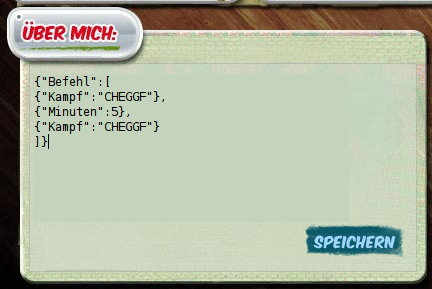
\includegraphics[width=8cm]{Beschreibung.png}
\end{center}

Seit der Version \texttt{1.0.beta5} gibt es eine Erweiterung hierzu. Der Platz in der Beschreibung ist begrenzt, also kann man Angriffe in einer einfachen Liste ausführen. Der folgende Befehl so direkt in die Beschreibung eingegeben, würde zwei Angriffe auf "\_wolf\_" ausführen, da die ID "CHEGGF", die von "\_wolf\_" ist.

\begin{code}[language=bash]
["CHEGGF","_wolf_"]
\end{code}

Ab Version \texttt{1.1.alpha3} ist es zusätzlich möglich, eine persönlich angepasste Beschreibung in den Plan anzugeben. Diese wird nach Abarbeitung der Befehle in die Beschreibung geschrieben. Wird diese nicht angegeben, schreibt das Programm immer \textit{Ich war bisher zu faul eine Beschreibung einzugeben, hole ich aber sicher bald nach!} in die Beschreibung.


\begin{code}[language=bash]
"Plan0":[
	{"Beschreibung":"Ich bin fertig mit den Aufgaben :)"}
],
\end{code} 


\subsection{Bank}
\label{Bank}
Der Befehl "Bank" bringt Geld auf die Sparkasse. Mit dem Parameter 0 bringt man so viel wie möglich auf die Bank. Mit allen anderen positiven Zahlen wird genauso viel Geld eingezahlt, welches von der Zahl repräsentiert wird.

\begin{code}[language=bash]
"Plan0":[
# Bringt alles auf die Bank
	{"Bank":0},
# Bringt nur 205 DM auf die Bank
	{"Bank":205}
],
\end{code}


\subsection{Befehl}
\label{PlanBefehl}
Der Befehl "Befehl" prüft ob ein Befehl vorliegt. Wird einer oder mehrere gefunden, wird immer der erste Abgearbeitet und danach wieder die Datei geöffnet um den nächsten zu suchen. Erst wenn alle Befehle abgearbeitet sind, wird die normale Ausführung fortgesetzt. Weitere Hinweise unter \nameref{Infopfad}.

\begin{code}[language=bash]
"Plan0":[
# Prüft ob ein neuer Befehl vorliegt
	{"Befehl":true}
],
\end{code}

\subsection{Booster}
\label{Booster}
Mit der Vereinsvitrine kam auch das Spiel "Booster" hinzu. Es kann mit folgenden Befehl ausgeführt werden. Funktioniert natürlich nur, wenn man am aktuellen Tag noch Booster ausführen darf.

\begin{code}[language=bash]
"Plan0":[
# Booster mit Ergebnis 5 ausführen
	{"Booster":5}
],
\end{code}


\subsection{Böse Spieler}
\label{Boese}
Der Befehl "Boese" greift eine Person aus der "Böse Spieler"-Liste an. Alle
Personen in der Liste werden gleichmäßig angegriffen. Pro Befehl wird ein
Angriff ausgeführt. (\textbf{Achtung}: In Version 1.0 hieß diese Funktion
"Böse", bis Version 1.2.3 hieß die Funktion dann "Boese")

Seitdem die Böseliste in drei Teile (Beute, Krieg, Respekt) aufgeteilt wurde,
gibt es die Möglichkeit auch nur eine Liste davon anzugreifen:

\begin{code}[language=bash]
"Plan0":[
# Beute-Liste-Person angreifen
	{"BoeseBeute":{}},
# Krieg-Liste-Person angreifen
	{"BoeseKrieg":{}},
# Respekt-Liste-Person angreifen
	{"BoeseRespekt":{}}
],
\end{code}

Es kann auch die \nameref{Medizin}-Option gesetzt werden.

Es kann auch die \nameref{Zwerg}-Option gesetzt werden.

\begin{code}[language=bash]
"Plan0":[
	{"BoeseRespekt":{"Medizin":40,"Zwerg":true}}
],
\end{code}

Seit der Version \texttt{1.2.5} gibt es die Möglichkeit einen Beutereichen
Gegner erneut anzugreifen. Dies geschieht ähnlich dem Prinzip beim normalen
\nameref{Angriff}. Man gibt mit der Option \texttt{nochmal} einen D-Mark-Betrag
an. Falls der bei einem Angriff erreicht wurde, wird bei dem nächsten Aufruf des
gleichen Planelements genau dieser Gegner nochmal angegriffen.

\begin{code}[language=bash]
"Plan0":[
# nochmal angreifen ab 40 D-Mark Beute
	{"BoeseRespekt":{"nochmal":40}}
],
\end{code}

\subsection{Goldene Zwerge}
\label{Golden}
Der Befehl "Golden" greift den nächsten Goldenen Zwerg an. Dabei ist diese Option nur Sinnvoll, wenn die Konfiguration mit der erweiterten Ausgabe eingestellt ist. Außerdem sollte man es nur in der Beschreibung benutzen.

\begin{code}[language=bash]
{"Befehl":[
	{"Golden":true}
]}
\end{code}


Es kann auch die \nameref{Medizin}-Option gesetzt werden.

\begin{code}[language=bash]
"Plan0":[
	{"Golden":{"Medizin":40}}
],
\end{code}

\subsection{Kampf}
\label{Kampf}
Der Befehl "Kampf" erzeugt im Gegensatz zu "Boese" und "Angriff" eine Keilerei mit einem bestimmten Gegner. Als Parameter wird entweder die ID oder der Name des Gegners übergeben. Die ID ist das Ende der URL, wenn man auf dem Profil ist. Bei der URL des Profils von "\_wolf\_" (1. Platz) lautet:\\
\texttt{http://www.bundeskampf.com/characters/profile/CHEGGF}\\
Die ID lautet also: \texttt{CHEGGF}
Man könnte auch den Namen angeben, allerdings wird der bei zu kurzen Namen nicht immer gefunden. Hier beide Beispiele:

\begin{code}[language=bash]
"Plan0":[
	{"Kampf":"CHEGGF"},
	{"Kampf":"_wolf_"}
],
\end{code}

Es kann auch die \nameref{Medizin}-Option gesetzt werden. Das feindliche Profil wird mit "\texttt{Gegner}" angegeben.

Es kann auch die \nameref{Zwerg}-Option gesetzt werden.

\begin{code}[language=bash]
"Plan0":[
	{"Kampf":{"Gegner":"_wolf_","Medizin":40,"Zwerg":true}}
],
\end{code}

\subsection{Minuten}
Der Befehl "Minuten" bewirkt ein Schlafen des Bots. Als Parameter nimmt er die Anzahl der Minuten, die er Schlafen soll. Dieser Befehl muss nicht für die anderen Funktionen benutzt werden, sondern ist dafür da, dass man selber etwas machen kann.

\begin{code}[language=bash]
"Plan0":[
# Warte 3 Minuten
	{"Minuten":3},
# Warte 2 Stunden
	{"Minuten":120}
],
\end{code}


\subsection{Neustart}
Will man an einer Stelle den internen Speicher säubern oder ist durch irgendeinen Bug genervt, kann man den Bot kontrolliert neu starten.

\begin{code}[language=bash]
"Plan0":[
	{"Neustart":true}
],
\end{code}


\subsection{Skill}

Dieses Element ermöglicht es das erworbene Geld direkt in einer Kategorie zu
skillen. Dafür wird es so benutzt:

\begin{code}[language=bash]
"Plan1":[
	{"Skill":{"Kategorie":"Mukkies"}},
	{"Skill":{"Kategorie":"Schleuderkraft"}},
	{"Skill":{"Kategorie":"Fitness"}},
	{"Skill":{"Kategorie":"Wahrnehmung"}},
	{"Skill":{"Kategorie":"Glueck"}}
],
\end{code}

Bei jeden Aufruf wird so oft wie möglich geskillt. Will man das nicht, muss man die maximale Anzahl angeben:

\begin{code}[language=bash]
"Plan1":[
	{"Skill":{"Kategorie":"Mukkies", "Anzahl":1}},
	{"Skill":{"Kategorie":"Schleuderkraft", "Anzahl":2}},
	{"Skill":{"Kategorie":"Fitness", "Anzahl":3}},
	{"Skill":{"Kategorie":"Wahrnehmung", "Anzahl":4}},
	{"Skill":{"Kategorie":"Glueck", "Anzahl":5}}
],
\end{code}

\subsection{Stopp}
Normalerweise arbeitet der Bot die Listen nacheinander ab und fängt wieder von vorne an. Um dies zu Unterbrechen gibt es den Befehl "Stopp".

\begin{code}[language=bash]
"Plan0":[
	{"Stopp":true}
],
\end{code}


\addtocontents{toc}{\protect\newpage}
\section{Programm-Varianten}

Das Programm implementiert verschiedene Hilfsmittel. Hier werden Sie aufgeführt und beschrieben.

\subsection{Tägliche Möglichkeiten}

Folgende tägliche Möglichkeiten können kombiniert werden. Maximal zu:

\begin{code}[emph={los,quiz,glueck,wein,spiel,jagd}]
eingabe# java -jar BKampfBot.jar los quiz glueck wein spiel jagd
\end{code}

Sie werden in der jeweiligen Reihenfolge mit nur einem Login ausgeführt.

\subsubsection{Tagesquiz}

Mit Hilfe des Programms kann das Tagesquiz ziemlich gut gelöst werden. Und es geht viel schneller, als wenn man es selber macht. Der Aufruf sieht wie folgt aus:

\begin{code}[emph={quiz}]
eingabe# java -jar BKampfBot.jar quiz
\end{code}

Die Fragen werden direkt (richtig) beantwortet. Sollen \textbf{nicht} alle Fragen richtig beantwortet werden\footnote{\url{https://warnow.mgvmedia.com/trac/BKampfBot/ticket/36}}, kann man auch angeben, wie viele Fragen \textbf{falsch} sein sollen:

\begin{code}[emph={quiz}]
eingabe# java -jar BKampfBot.jar quiz=2
\end{code}

\subsubsection{Rubbelos}

Wer schon mal selber versucht hat, die Rubbellose von ihrer Beschichtung zu befreien, der lässt es sehr schnell sein, denn es dauert zu lange. Will man es schneller erledigen, nimmt man folgenden Befehl:

\begin{code}[emph={los}]
eingabe# java -jar BKampfBot.jar los
\end{code}

\subsubsection{Glücksrad}
Diese Option funktioniert nur in einem Verein. Sie dreht das Rad auf die Gewinnposition.

\begin{code}[emph={glueck}]
eingabe# java -jar BKampfBot.jar glueck
\end{code}


\subsubsection{Weinkeller}
Diese Option funktioniert nur in einem Verein. Sie spielt das Weinkellerspiel und gewinnt es.

\begin{code}[emph={wein}]
eingabe# java -jar BKampfBot.jar wein
\end{code}


\subsubsection{Tagesspiel}
Das Tagesspiel wird mit voller Punktzahl ausgeführt.

\begin{code}[emph={spiel}]
eingabe# java -jar BKampfBot.jar spiel
\end{code}


\subsubsection{Wörterjagd}
\label{jagd}
Die Wörterjagd wird ausgeführt, bis man keine Punkte mehr hat. 

\begin{code}[emph={jagd}]
eingabe# java -jar BKampfBot.jar jagd
\end{code}

Dabei werden alle Begriffe sofort gelöst, außer man gibt folgende Konfiguration ein:

\begin{code}[language=bash]
"jagd":{
	"min":1,
	"max":5
},
\end{code}

Es wird dann zufällig gewählt, wie viele Buchstaben (zwischen 1 und 5) gewählt
werden, bis automatisch die richtige Lösung eingeben wird.

\subsection{Lottoschein}
\textit{Genau wie im Fernsehen könnt ihr es euch Sonntags Abend gemütlich machen und darauf hoffen, dass die Glücksfee euch diese Woche hold ist. Und ihr - zumindest in Bundeskampf - nicht mehr zu arbeiten braucht.}

Das Ausfüllen eines Scheins dauert auch ein wenig. Und welche Zahlen soll man nehmen? Mit dem folgenden Aufruf erledigt es das Programm:

\begin{code}[emph={lotto}]
eingabe# java -jar BKampfBot.jar lotto
\end{code}

Beispielausgabe (die Zahlen werden zufällig gewählt):

\begin{code}[basicstyle=\tiny\ttfamily]
Login
visit: http://www.bundeskampf.com/lotto/history
Added numbers: 2,5,10,38,40
Logout
visit: http://www.bundeskampf.com/signups/logout
\end{code}

Ab Version \texttt{1.1.alpha6} kann man die Nummern auch direkt angeben:

\begin{code}[emph={lotto}]
eingabe# java -jar BKampfBot.jar lotto=12,34,23,45,2
\end{code}

\subsection{Testen des Proxy}
\label{proxytest}

Mit der Option \texttt{testproxy} wird eine Webseite aufgerufen, die nur die IP
zurückgibt. Diese kann man dann mit der originalen IP vergleichen.

\begin{code}[emph={testproxy}]
eingabe# java -jar BKampfBot.jar testproxy
Deine IP: 1.2.3.4
\end{code}


\section{Weitere Hinweise}
\subsection{Medizin}
\label{Medizin}
Man kann bei verschiedenen Optionen die Wartezeit verkürzen, indem man Medizin kauft. Im Spiel wird diese "Direkt Fit" genannt. Folgende Pläne benutzen die Aktion: \nameref{Angriff}, \nameref{Aussendienst}, \nameref{Boese}, \sout{\nameref{Golden}} und \nameref{Kampf}.

In der Konfiguration gibt man eine ganzstellige Zahl an, die als Prozent der restlichen Lebensenergie angesehen wird, ab der Medizin gekauft wird. Die Rechnung lautet: 

$$\frac{Lebenspunkte}{Maximale Lebenspunkte}=Prozent$$

Am besten ein Beispiel zur Anschauung. Jemand hat folgenden Plan eingetragen:

\begin{code}[language=bash,emph={Medizin}]
"Plan0":[
	{"Angriff":{"Stufe":0,"Verein":0,"Medizin":40}}
],
\end{code}

Es soll also Medizin gekauft werden, wenn nach dem Kampf die Lebensenergie unter $40\%$ gefallen ist. Nun kämpft er und erhält folgendes Ergebnis:

$$\frac{345LP}{1000LP} = 35\%$$

Die Medizin wird also gekauft. 

Trägt man 0 ein, wird gekauft, wenn man den Kampf verloren hat und die Lebenspunkte komplett runter sind. Wird 100 eingetragen, wird die Medizin immer gekauft.


\subsection{Zwerge geben}
\label{Zwerg}
Man kann bei den Kämpfen die Wartezeit auflösen, indem man einen Zwerg einsetzt.
Deswegen gibt es ab Version \texttt{1.2.7} die Möglichkeit dies anzugeben. Dafür
gibt man einfach die Option mit an:

\begin{code}[language=bash,emph={Medizin}]
"Plan0":[
	{"Angriff":{"Stufe":0,"Verein":0,"Medizin":40,"Zwerg":true}}
],
\end{code}

Wenn nun zu dem Zeitpunkt ein Zwerg eingelöst werden kann, wird die Wartezeit
verkürzt und keine Medizin gekauft. Sollten keine Zwerge mehr da sein, wird in
diesem Fall die Medizin gekauft.



\subsection{Vorausschauende Pläne}
\label{Vorausschauen}

Ab Version \texttt{1.1.alpha6} ermöglichen ein neuer Planmanager das vorausschauen von Aktionen. Innerhalb der Kampfwartezeit kann somit zum Beispiel schon ein Außendienst gestartet werden, falls er im Plan an nächster Stelle folgt. 

Folgende Pläne werden früher gestartet:
\begin{itemize}
  \item \nameref{Arbeiten}
  \item \nameref{Aussendienst}
  \item \nameref{Bank}
  \item \nameref{Booster}
\end{itemize}

Folgende Pläne ermöglichen ein vorzeitiges Abarbeiten in der Wartezeit:
\begin{itemize}
  \item \nameref{Angriff}
  \item \nameref{Boese}
  \item \nameref{Golden}
  \item \nameref{Kampf}
\end{itemize}

Um diese Funktionalität zu deaktivieren benötigt man folgenden Befehl in der Konfiguration:

\begin{code}[language=bash]
"Benutzername":"meinName",
"Passwort":"geheim",
"Vorausschauen":false,
[...]
\end{code}


\subsection{Useragent}
\label{Useragent}

Ein Programm sendet im Internet meistens einen Hinweis auf die eigene Version an die Webserver. Browser machen das auch. Deshalb sendet der Bot auch einen Useragent, der genauso aussieht, wie der eines Firefoxes oder Internet-Explorers. Mit der Option \texttt{Useragent} kann man seinen eigenen Useragent setzen um einen anderen Browser vorzutäuschen.

\begin{code}[language=bash,basicstyle=\tiny\ttfamily]
[...]
"Useragent":"Mozilla/5.0 (Windows; U; Windows NT 5.1; de; rv:1.9.0.10) Gecko/2009042316 Firefox/3.0.10",
[...]
\end{code}

\subsection{Zeitfaktor}
\label{Zeitfaktor}

Mittels der Option \texttt{Zeitfaktor} kann man die zeitliche Abarbeitung des Bots beeinflussen. Im Programm sind an einigen wiederkehrenden Stellen Haltepositionen eingebaut. An diesesen Stellen `schläft` das Programm für eine bestimmte Zeit, bevor es die Abarbeitung fortsetzt. Mit dem Zeitfaktor kann man diese Zeit um den angegeben Faktor verlängern.

Der Faktor wird an die vorgegebene Zeit angepasst. Schläft der Bot länger als eine Minute, wird der Faktor ignoriert. 

\begin{code}
Hole http://example.com/1.html
Schlafe (10 Millisekunden * Faktor)
Hole http://example.com/2.html
Schlafe (10 Millisekunden * Faktor)
\end{code}

Den Faktor kann man nun auf zwei Arten einstellen, entweder mit einem festen Wert oder mit einem Intervall, indem bei jedem Anwenden zufällig ein Wert daraus genommen wird.

\begin{code}[language=bash]
[...]
# fest
"Zeitfaktor":20,

# Intervall
"Zeitfaktor":{"min":20, "max": 100},
[...]
\end{code}

Durch diese Option kann der Bot sehr individuell gestaltet werden. Ein höherer Wert lässt den Bot langsamer arbeiten, wodurch aber ein geringeres Entdeckungsrisiko gegeben ist.

\subsection{Proxy}
\label{Proxy}

Ab der Version 1.2.3 ist es möglich einen Proxy zu benutzen. Dafür ist zwingend
die Angabe von Hostname und Port erforderlich. Falls eine Anmeldung bei dem
Proxy erforderlich ist, kann der Benutzername und das Passwort angegeben werden.

\begin{code}[language=bash]
[...]
# Proxy ohne Authentifizierung
"Proxy":{
	"Host":"IP oder Domain",
	"Port":8080
},
[...]
\end{code}

\begin{code}[language=bash]
[...]
# Proxy mit Authentifizierung
"Proxy":{
	"Host":"IP oder Domain",
	"Port":8080,
	"Username": "username",
	"Password": "password"
},
[...]
\end{code}

Um das ganze zu Testen gibt es die Option \nameref{proxytest}.

\subsection{Verschleiern des Bots}
\label{Verschleiern}

Angelehnt auf die Anfrage von
"Xanadou"\footnote{\url{https://warnow.mgvmedia.com/trac/BKampfBot/ticket/52}}
wurde eine neue Funktion in den Bot aufgenommen. Wenn der Bot eine längere Zeit
warten muss, werden zufällig Seiten aufgerufen, die ein Mensch auch aufrufen
würde.

Ein Beispiel zur Veranschaulichung:

Der Bot soll einen Außendienst machen. Er erledigt das. Dabei muss er eine halbe
Stunde warten. In dieser Zeit wählt er zufällig aus, dass er nach den letzten
Lottozahlen gucken soll. Also ruft er das "Fleißhelft" auf und dann die
"Lottoscheine". Falls danach noch Zeit ist ruft er wieder eine ähliche Abfolge
auf.

Da mir nocht nicht genügend Abfolgen zugesandt wurden, ist die Funktion noch
nicht standardmäßig aktiv. Mann kann sie aber mit der Config-Option
"Verschleiern" aktivieren:

\begin{code}[language=bash]
[...]
# Verschleiern aktivieren
"Verschleiern":true,
[...]
\end{code}

\subsection{Erweitere Ausgabe und Befehle}
\label{Infopfad}

Durch die Angabe der Config-Option \texttt{"Info Pfad"}, kann man ein Verzeichnis bestimmen, in dem eine erweiterte Ausgabe abgespeichert wird. Für jeden Kampf wird dort eine HTML-Datei mit Einzelheiten zum Verlauf gespeichert. 

Legt man ein in diesem angegebenen Verzeichnis ein weiteres Verzeichnis mit dem Namen \texttt{befehl} an, hat man mit dem \hyperref[PlanBefehl]{Plan Befehl} weitere Möglichkeiten. Sobald der Bot zum diesem Planelement kommt, wird die Datei \texttt{befehl.json} abgearbeitet. In dieser Datei ist ein JSON-Objekt mit weiteren Planelementen enthalten. Sobald ein Element abgearbeitet ist, wird es aus der Datei gelöscht. Der Inhalt von \texttt{befehl.json} sieht zum Beispiel so aus:

\begin{code}[language=bash]
{
	"Befehl":[
		{"Kampf":"CHEGGF"},
		{"Kampf":"CHEGGF"},
		{"Kampf":"CHEGGF"}
	]
}
\end{code}

\subsection{Unerwartete Fehler}
Sollte ein unerwarteter Fehler auftreten, welches zu einem Absturz des Systems führt, wird der Fehler mit mehreren Hinweisen ausgegeben. Danach startet sich das Programm neu. Das Programm versucht dann erneut seine Aufgaben zu erledigen. Passiert zu oft ein Absturz beendet sich das Programm.

Sollten Sie sich den Fehler durch die Ausgaben des Bots und durch selbstständigen Prüfen auf der Webseite nicht erklären lassen, wird darum gebeten ein Ticket auf der Entwicklerseite\footnote{\url{https://warnow.mgvmedia.com/trac/BKampfBot/newticket}} zu erstellen. Dort können auch Wünsche für neue Funktionen geäußert werden.

\subsubsection{Bekannte Fehler}
Tritt ein Fehler auf, in dem von einem \textit{Internal Server Error - 500} die Rede ist, liegt es an dem Bundeskampf-Server und nicht am Bot. Die genaue Fehlermeldung ist auf der Webseite zu finden.


\section{Beispielkonfigurationen}
\label{example}
Die folgenden Konfigurationen sind auch auf der Webseite zum Download verfügbar.

Eine Konfiguration für jemanden, der nur die Außendienste (schwer) machen will und danach das Programm beenden will, sieht dann so aus:

\begin{code}[language=bash]
"Benutzername":"meinName",
"Passwort":"geheim",
"Plan0":[
	{"Aussendienst":1}
],
"Plan1":[
	{"Stopp":true}
]
\end{code}


Konfiguration: Nur Außendienste leicht, wenn fertig, regelmäßig prüfen, ob es schon ein neuer Tag ist und dann wieder Außendienste machen:

\begin{code}[language=bash]
"Benutzername":"meinName",
"Passwort":"geheim",
"Plan0":[
	{"Aussendienst":0}
],
"Plan1":[
	{"Minuten":30}
]
\end{code}

Konfiguration: Keine Außendienste; Nur Angreifen, gleiche Stufe, im Verein.

\begin{code}[language=bash]
"Benutzername":"meinName",
"Passwort":"geheim",
"Plan1":[
	{"Angriff":{"Stufe":0,"Verein":1}}
]
\end{code}

Konfiguration: Keine Außendienste; Nur Arbeiten, dann alles auf Bank bringen.

\begin{code}[language=bash]
"Benutzername":"meinName",
"Passwort":"geheim",
"Plan1":[
	{"Arbeiten":1},
	{"Bank":0}
]
\end{code}

Konfiguration: Keine Außendienste; Angreifen, dann einen bösen Angreifen und dann eine Pause.

\begin{code}[language=bash]
"Benutzername":"meinName",
"Passwort":"geheim",
"Plan1":[
	{"Angriff":{"Stufe":0,"Verein":1}},
	{"Boese":1},
	{"Minuten":10}
]
\end{code}
\ccbyncsa
\end{document} 
